% ETH Zurich  - 3D Photography 2015
% http://www.cvg.ethz.ch/teaching/3dphoto/
% Template for project proposals

\documentclass[11pt,a4paper,oneside,onecolumn]{IEEEtran}
\usepackage{graphicx}
\usepackage{caption}
% Enter the project title and your project supervisor here
\newcommand{\ProjectTitle}{SfM from RGB-D data}
\newcommand{\ProjectSupervisor}{Bernhard Zeisl}
\newcommand{\DateOfReport}{March 6, 2015}

% Enter the team members' names and path to their photos. Comment / uncomment related definitions if the number of members are different than 2.
% Including photographs are optional. Photos are there to help us to evaluate your group more effectively. If you wish not to include your photos, please comment the following line.
\newcommand{\PutPhotos}{}
% Please include a clear photo of each member. (use pdf or png files for Latex to embed them in the document well)
\newcommand{\memberone}{Seonwook Park}
\newcommand{\memberonepicture}{pic2.png}
\newcommand{\membertwo}{Yifan Wang}
\newcommand{\membertwopicture}{pic1.png}
%\newcommand{\memberthree}{Member Name}
%\newcommand{\memberthreepicture}{pic3.png}


%%%% DO NOT EDIT THE PART BELOW %%%%
\title{\ProjectTitle}
\author{3D Photography Project Proposal\\Supervised by: \ProjectSupervisor\\ \DateOfReport}
\begin{document}
\maketitle
\vspace{-1.5cm}\section*{Group Members}\vspace{0.3cm}
\begin{center}\begin{minipage}{\linewidth}\begin{center}
\begin{minipage}{3 cm}\begin{center}\memberone\ifdefined\PutPhotos\\\vspace{0.2cm}\includegraphics[height=3cm]{\memberonepicture}\fi\end{center}\end{minipage}
\ifdefined\membertwo\begin{minipage}{3 cm}\begin{center}\membertwo\ifdefined\PutPhotos\\\vspace{0.2cm}\includegraphics[height=3cm]{\membertwopicture}\fi\end{center}\end{minipage}\fi
\ifdefined\memberthree\begin{minipage}{3 cm}\begin{center}\memberthree\ifdefined\PutPhotos\\\vspace{0.2cm}\includegraphics[height=3cm]{\memberthreepicture}\fi\end{center}\end{minipage}\fi
\end{center}\end{minipage}\end{center}\vspace{0.3cm}
%%%% END OF PROTECTED LINES %%%%


%%%% BEGIN WRITING THE DOCUMENT HERE %%%%

\section{Description of the project}

This project aims to reconstruct a 3D model of an environment using structure
from motion (SfM). A pipeline will be assembled which makes use of depth data
taken from a Kinect \cite{reckerdepth}. Our work is devoted to investigating
how depth information can simplify the scene registration step and improve
accuracy of the final reconstructed model.

\section{Work packages and timeline}

First, a small base dataset will be acquired using a Kinect. A basic pipeline
will be assembled where (i) SURF/SIFT features are detected (ii) then matched to
find coarse estimations of camera pose (iii) then a final step where a finer
estimate of the scene is found.

We aim to follow the following timeline:

\def\arraystretch{1.5}
\vspace{1em}
\begin{tabular}{|r|p{.82\columnwidth}|}
	\hline
	22nd March &
	Acquisition of small initial dataset using the Kinect. \newline
	Review and planning of specifics of the pipeline implementation.
	\\
	\hline
	2nd April &
	Feature extraction from acquired images using $\mathrm{vlfeat}$ and
	matching of image pairs or triples.
	\\
	\hline
	24th April &
	Coarse estimation of camera and feature pose and initial visualization
	using $\mathrm{PCL}$.
	\\
	\hline
	8th May &
	Finer estimation of feature pose via Bundle Adjustment using
	$\mathrm{ceres}$.
	\\
	\hline
	22nd May &
	Implementation of alternate scene registration methods. Evaluation of
	results.
	\\
	\hline
\end{tabular}
\vspace{1em}

A challenge is the evaluation of various scene registration methods, including
2D-2D, 3D-3D and 3D-2D point registration. Furthermore a suitable global
optimizer is to be found, which incorporates sensor’s depth information as
prior.

The implementation will mainly be carried out using C++. Various libraries will
be used, such as vlfeat (feature detection),  PnP solvers (scene registration),
and ceres (bundle adjustment).

\section{Outcomes and Demonstration}

The project should yield a 3D reconstruction of a room environment. This
procedure can be verified by applying to an unknown scene. A visualization of
the result will be shown using the Point Cloud Library (PCL) or Meshlab, with
comparisons to a video feed.


%\vspace{1cm}
%\textbf{Instructions:}
%
%\begin{itemize}
%\item The document should not exceed two pages including the references.
%\item Please name the document \textbf{3DPhoto\_Proposal\_Surname1\_Surname2.pdf} and send it to Ya\u{g}{\i}z in an email titled \textbf{[3DPhoto] Project Proposal - Surname1 Surname2}, filling in your surnames.
%\end{itemize}

\begin{figure}[h!]
\begin{center}
	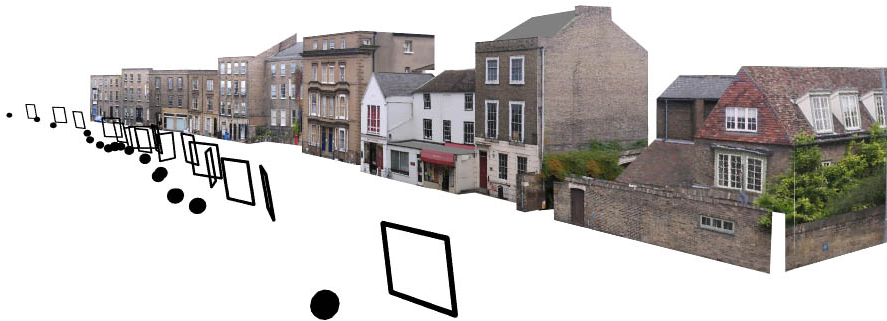
\includegraphics[width=.5\textwidth]{img.png}
	\caption{A 3D reconstruction of houses on a street\cite{varga2008practical}}
\end{center}
\end{figure}

{%\singlespace
{\small
\bibliography{refs}
\bibliographystyle{plain}}}




\end{document}
